% Options for packages loaded elsewhere
\PassOptionsToPackage{unicode}{hyperref}
\PassOptionsToPackage{hyphens}{url}
%
\documentclass[
]{article}
\usepackage{lmodern}
\usepackage{amssymb,amsmath}
\usepackage{ifxetex,ifluatex}
\ifnum 0\ifxetex 1\fi\ifluatex 1\fi=0 % if pdftex
  \usepackage[T1]{fontenc}
  \usepackage[utf8]{inputenc}
  \usepackage{textcomp} % provide euro and other symbols
\else % if luatex or xetex
  \usepackage{unicode-math}
  \defaultfontfeatures{Scale=MatchLowercase}
  \defaultfontfeatures[\rmfamily]{Ligatures=TeX,Scale=1}
\fi
% Use upquote if available, for straight quotes in verbatim environments
\IfFileExists{upquote.sty}{\usepackage{upquote}}{}
\IfFileExists{microtype.sty}{% use microtype if available
  \usepackage[]{microtype}
  \UseMicrotypeSet[protrusion]{basicmath} % disable protrusion for tt fonts
}{}
\makeatletter
\@ifundefined{KOMAClassName}{% if non-KOMA class
  \IfFileExists{parskip.sty}{%
    \usepackage{parskip}
  }{% else
    \setlength{\parindent}{0pt}
    \setlength{\parskip}{6pt plus 2pt minus 1pt}}
}{% if KOMA class
  \KOMAoptions{parskip=half}}
\makeatother
\usepackage{xcolor}
\IfFileExists{xurl.sty}{\usepackage{xurl}}{} % add URL line breaks if available
\IfFileExists{bookmark.sty}{\usepackage{bookmark}}{\usepackage{hyperref}}
\hypersetup{
  pdftitle={Statistical Inference Course Project},
  pdfauthor={Kaaltho},
  hidelinks,
  pdfcreator={LaTeX via pandoc}}
\urlstyle{same} % disable monospaced font for URLs
\usepackage[margin=1in]{geometry}
\usepackage{color}
\usepackage{fancyvrb}
\newcommand{\VerbBar}{|}
\newcommand{\VERB}{\Verb[commandchars=\\\{\}]}
\DefineVerbatimEnvironment{Highlighting}{Verbatim}{commandchars=\\\{\}}
% Add ',fontsize=\small' for more characters per line
\usepackage{framed}
\definecolor{shadecolor}{RGB}{248,248,248}
\newenvironment{Shaded}{\begin{snugshade}}{\end{snugshade}}
\newcommand{\AlertTok}[1]{\textcolor[rgb]{0.94,0.16,0.16}{#1}}
\newcommand{\AnnotationTok}[1]{\textcolor[rgb]{0.56,0.35,0.01}{\textbf{\textit{#1}}}}
\newcommand{\AttributeTok}[1]{\textcolor[rgb]{0.77,0.63,0.00}{#1}}
\newcommand{\BaseNTok}[1]{\textcolor[rgb]{0.00,0.00,0.81}{#1}}
\newcommand{\BuiltInTok}[1]{#1}
\newcommand{\CharTok}[1]{\textcolor[rgb]{0.31,0.60,0.02}{#1}}
\newcommand{\CommentTok}[1]{\textcolor[rgb]{0.56,0.35,0.01}{\textit{#1}}}
\newcommand{\CommentVarTok}[1]{\textcolor[rgb]{0.56,0.35,0.01}{\textbf{\textit{#1}}}}
\newcommand{\ConstantTok}[1]{\textcolor[rgb]{0.00,0.00,0.00}{#1}}
\newcommand{\ControlFlowTok}[1]{\textcolor[rgb]{0.13,0.29,0.53}{\textbf{#1}}}
\newcommand{\DataTypeTok}[1]{\textcolor[rgb]{0.13,0.29,0.53}{#1}}
\newcommand{\DecValTok}[1]{\textcolor[rgb]{0.00,0.00,0.81}{#1}}
\newcommand{\DocumentationTok}[1]{\textcolor[rgb]{0.56,0.35,0.01}{\textbf{\textit{#1}}}}
\newcommand{\ErrorTok}[1]{\textcolor[rgb]{0.64,0.00,0.00}{\textbf{#1}}}
\newcommand{\ExtensionTok}[1]{#1}
\newcommand{\FloatTok}[1]{\textcolor[rgb]{0.00,0.00,0.81}{#1}}
\newcommand{\FunctionTok}[1]{\textcolor[rgb]{0.00,0.00,0.00}{#1}}
\newcommand{\ImportTok}[1]{#1}
\newcommand{\InformationTok}[1]{\textcolor[rgb]{0.56,0.35,0.01}{\textbf{\textit{#1}}}}
\newcommand{\KeywordTok}[1]{\textcolor[rgb]{0.13,0.29,0.53}{\textbf{#1}}}
\newcommand{\NormalTok}[1]{#1}
\newcommand{\OperatorTok}[1]{\textcolor[rgb]{0.81,0.36,0.00}{\textbf{#1}}}
\newcommand{\OtherTok}[1]{\textcolor[rgb]{0.56,0.35,0.01}{#1}}
\newcommand{\PreprocessorTok}[1]{\textcolor[rgb]{0.56,0.35,0.01}{\textit{#1}}}
\newcommand{\RegionMarkerTok}[1]{#1}
\newcommand{\SpecialCharTok}[1]{\textcolor[rgb]{0.00,0.00,0.00}{#1}}
\newcommand{\SpecialStringTok}[1]{\textcolor[rgb]{0.31,0.60,0.02}{#1}}
\newcommand{\StringTok}[1]{\textcolor[rgb]{0.31,0.60,0.02}{#1}}
\newcommand{\VariableTok}[1]{\textcolor[rgb]{0.00,0.00,0.00}{#1}}
\newcommand{\VerbatimStringTok}[1]{\textcolor[rgb]{0.31,0.60,0.02}{#1}}
\newcommand{\WarningTok}[1]{\textcolor[rgb]{0.56,0.35,0.01}{\textbf{\textit{#1}}}}
\usepackage{graphicx,grffile}
\makeatletter
\def\maxwidth{\ifdim\Gin@nat@width>\linewidth\linewidth\else\Gin@nat@width\fi}
\def\maxheight{\ifdim\Gin@nat@height>\textheight\textheight\else\Gin@nat@height\fi}
\makeatother
% Scale images if necessary, so that they will not overflow the page
% margins by default, and it is still possible to overwrite the defaults
% using explicit options in \includegraphics[width, height, ...]{}
\setkeys{Gin}{width=\maxwidth,height=\maxheight,keepaspectratio}
% Set default figure placement to htbp
\makeatletter
\def\fps@figure{htbp}
\makeatother
\setlength{\emergencystretch}{3em} % prevent overfull lines
\providecommand{\tightlist}{%
  \setlength{\itemsep}{0pt}\setlength{\parskip}{0pt}}
\setcounter{secnumdepth}{-\maxdimen} % remove section numbering

\title{Statistical Inference Course Project}
\author{Kaaltho}
\date{20/12/2020}

\begin{document}
\maketitle

\hypertarget{synopsis}{%
\subsubsection{Synopsis}\label{synopsis}}

The exponential distribution is going to be simulated in R with rexp(n,
lambda) where lambda is the rate parameter. The mean of exponential
distribution is 1/lambda and the standard deviation is also 1/lambda.
The parameter lambda is set to 0.2 for all of the simulations. This
investigation considers the distribution of averages of 40 exponential.

\hypertarget{part-1-simulation-exercise}{%
\subsubsection{\texorpdfstring{\textbf{Part 1: Simulation
Exercise}}{Part 1: Simulation Exercise}}\label{part-1-simulation-exercise}}

The first step is to simulate the variables that we want to compare.

\begin{Shaded}
\begin{Highlighting}[]
\CommentTok{#Oppening libraries}
\KeywordTok{library}\NormalTok{(ggplot2)}

\CommentTok{#Assigning variables names, the specified data is the following:}
\NormalTok{lambda <-}\StringTok{ }\FloatTok{0.2}
\NormalTok{n <-}\StringTok{ }\DecValTok{40}
\NormalTok{simulations <-}\StringTok{ }\DecValTok{1}\OperatorTok{:}\DecValTok{1000}
\KeywordTok{set.seed}\NormalTok{(}\DecValTok{100}\NormalTok{)}

\CommentTok{# Simulate the population}
\NormalTok{population <-}\StringTok{ }\KeywordTok{data.frame}\NormalTok{(}\DataTypeTok{x=}\KeywordTok{sapply}\NormalTok{(simulations, }\ControlFlowTok{function}\NormalTok{(x) \{}\KeywordTok{mean}\NormalTok{(}\KeywordTok{rexp}\NormalTok{(n, lambda))\}))}

\CommentTok{#The random varaibles looks like this:}
\KeywordTok{head}\NormalTok{(population)}
\end{Highlighting}
\end{Shaded}

\begin{verbatim}
##          x
## 1 4.137412
## 2 6.051703
## 3 4.415869
## 4 4.404714
## 5 3.210413
## 6 5.475307
\end{verbatim}

The next plot contains the distribution of the variables and it is
possible to see if it follows some distribution.

\begin{Shaded}
\begin{Highlighting}[]
\KeywordTok{ggplot}\NormalTok{(population, }\KeywordTok{aes}\NormalTok{(}\DataTypeTok{x=}\NormalTok{x)) }\OperatorTok{+}\StringTok{ }
\StringTok{  }\KeywordTok{geom_histogram}\NormalTok{(}\KeywordTok{aes}\NormalTok{(}\DataTypeTok{y=}\NormalTok{..count.., }\DataTypeTok{fill=}\NormalTok{..count..),}\DataTypeTok{color=}\StringTok{"skyblue"}\NormalTok{) }\OperatorTok{+}
\StringTok{  }\KeywordTok{guides}\NormalTok{(}\DataTypeTok{fill=}\OtherTok{FALSE}\NormalTok{) }\OperatorTok{+}
\StringTok{  }\KeywordTok{labs}\NormalTok{(}\DataTypeTok{title=}\StringTok{"Averages of 40 Exponentials for 1000 Simulations"}\NormalTok{, }\DataTypeTok{y=}\StringTok{"Frequency"}\NormalTok{, }\DataTypeTok{x=}\StringTok{"Mean"}\NormalTok{)}\OperatorTok{+}
\StringTok{  }\KeywordTok{theme}\NormalTok{(}\DataTypeTok{plot.title =} \KeywordTok{element_text}\NormalTok{(}\DataTypeTok{hjust =} \FloatTok{0.5}\NormalTok{))}
\end{Highlighting}
\end{Shaded}

\begin{verbatim}
## `stat_bin()` using `bins = 30`. Pick better value with `binwidth`.
\end{verbatim}

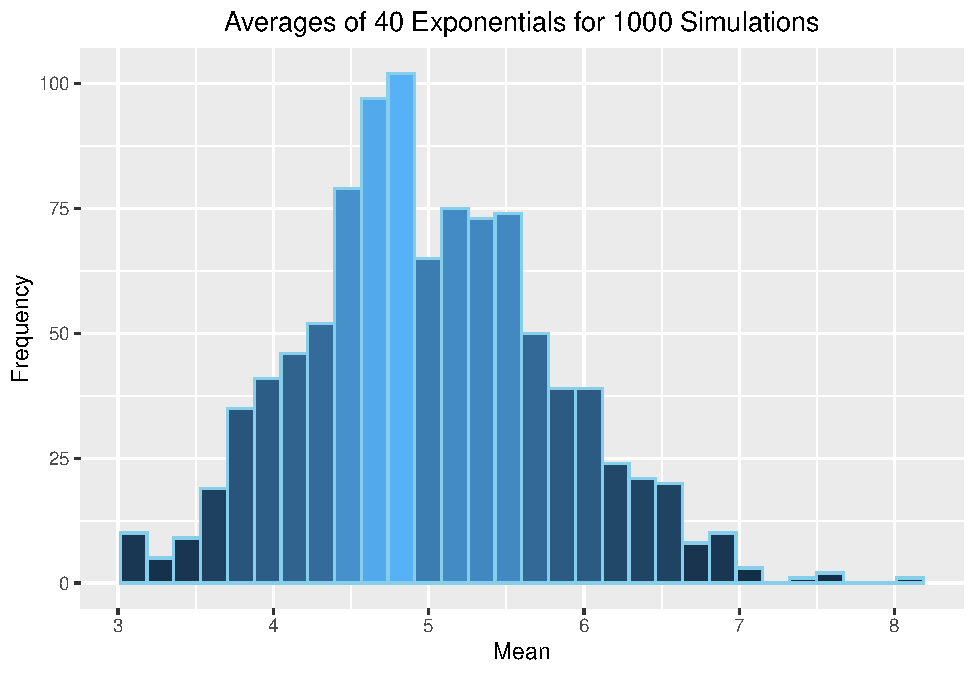
\includegraphics{Statistical-Inference-Course-Project_files/figure-latex/simulation2-1.pdf}

It is possible to see how the data accumulates near 5, and also the
shape of the data seems to be similar to a normal distribution.

\textbf{\emph{Show the sample mean and compare it to the theoretical
mean of the distribution.}}

\begin{Shaded}
\begin{Highlighting}[]
\CommentTok{# The mean and the theoretical mean of the distribution is as following:}
\NormalTok{sample.mean <-}\StringTok{ }\KeywordTok{mean}\NormalTok{(population}\OperatorTok{$}\NormalTok{x)}
\NormalTok{theoretical.mean <-}\StringTok{ }\DecValTok{1}\OperatorTok{/}\NormalTok{lambda}
\end{Highlighting}
\end{Shaded}

The sample mean is 4.9997019 and compare the theoretical mean is 5

\textbf{\emph{Show how variable the sample is (via variance) and compare
it to the theoretical variance of the distribution.}}

\begin{Shaded}
\begin{Highlighting}[]
\NormalTok{sample.variance <-}\StringTok{ }\KeywordTok{var}\NormalTok{(population)}
\NormalTok{theoretical.variance  <-}\StringTok{ }\NormalTok{(}\DecValTok{1} \OperatorTok{/}\StringTok{ }\NormalTok{lambda)}\OperatorTok{^}\DecValTok{2} \OperatorTok{/}\StringTok{ }\NormalTok{(n) }


\NormalTok{sample.sd <-}\StringTok{ }\KeywordTok{sd}\NormalTok{(population}\OperatorTok{$}\NormalTok{x)}
\NormalTok{theoretical.sd  <-}\StringTok{ }\DecValTok{1}\OperatorTok{/}\NormalTok{(lambda }\OperatorTok{*}\StringTok{ }\KeywordTok{sqrt}\NormalTok{(n))}
\end{Highlighting}
\end{Shaded}

\textbf{\emph{Show that the distribution is approximately normal.}}

\begin{Shaded}
\begin{Highlighting}[]
\KeywordTok{ggplot}\NormalTok{(population, }\KeywordTok{aes}\NormalTok{(}\DataTypeTok{x=}\NormalTok{x)) }\OperatorTok{+}
\StringTok{  }\KeywordTok{geom_histogram}\NormalTok{(}\KeywordTok{aes}\NormalTok{(}\DataTypeTok{y=}\NormalTok{..density..), }\DataTypeTok{colour=}\StringTok{"darkviolet"}\NormalTok{, }\DataTypeTok{fill=}\StringTok{"skyblue"}\NormalTok{)}\OperatorTok{+}\StringTok{ }
\StringTok{  }\KeywordTok{guides}\NormalTok{(}\DataTypeTok{fill=}\OtherTok{FALSE}\NormalTok{) }\OperatorTok{+}
\StringTok{  }\KeywordTok{labs}\NormalTok{(}\DataTypeTok{x=}\StringTok{"Quantity"}\NormalTok{, }\DataTypeTok{y=}\StringTok{"Density"}\NormalTok{, }\DataTypeTok{title=}\NormalTok{(}\StringTok{"Measn distribution for 40 samples"}\NormalTok{))}\OperatorTok{+}
\StringTok{  }\KeywordTok{theme}\NormalTok{(}\DataTypeTok{plot.title =} \KeywordTok{element_text}\NormalTok{(}\DataTypeTok{hjust =} \FloatTok{0.5}\NormalTok{)) }\OperatorTok{+}
\StringTok{  }\KeywordTok{geom_vline}\NormalTok{(}\KeywordTok{aes}\NormalTok{(}\DataTypeTok{xintercept=}\NormalTok{sample.mean, }\DataTypeTok{colour=}\StringTok{"Sample"}\NormalTok{))}\OperatorTok{+}
\StringTok{  }\KeywordTok{geom_vline}\NormalTok{(}\KeywordTok{aes}\NormalTok{(}\DataTypeTok{xintercept=}\NormalTok{theoretical.mean, }\DataTypeTok{colour=}\StringTok{"Theoretical"}\NormalTok{))}\OperatorTok{+}
\StringTok{  }\KeywordTok{stat_function}\NormalTok{(}\DataTypeTok{fun=}\NormalTok{dnorm, }\DataTypeTok{args=}\KeywordTok{list}\NormalTok{(}\DataTypeTok{mean=}\NormalTok{sample.mean,}\DataTypeTok{sd=}\NormalTok{sample.sd), }\DataTypeTok{color=}\StringTok{"purple3"}\NormalTok{)}\OperatorTok{+}
\StringTok{  }\KeywordTok{stat_function}\NormalTok{(}\DataTypeTok{fun=}\NormalTok{dnorm, }\DataTypeTok{args=}\KeywordTok{list}\NormalTok{(}\DataTypeTok{mean=}\NormalTok{theoretical.mean, }\DataTypeTok{sd=}\NormalTok{theoretical.sd), }\DataTypeTok{color=}\StringTok{"yellowgreen"}\NormalTok{)}
\end{Highlighting}
\end{Shaded}

\begin{verbatim}
## `stat_bin()` using `bins = 30`. Pick better value with `binwidth`.
\end{verbatim}

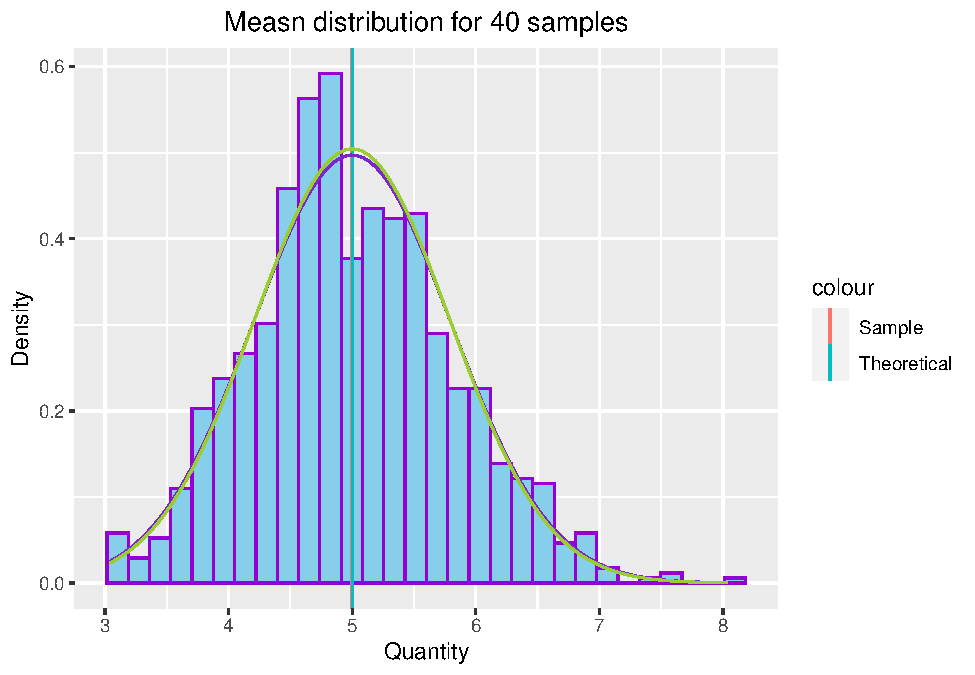
\includegraphics{Statistical-Inference-Course-Project_files/figure-latex/plot-1.pdf}

As is shown in the plot, the sample mean and the theoretical mean
overlaps, from the shape of the plot it can be say that the distribution
of means of 40 exponential distributions is close to the normal
distribution.

\end{document}
